% Created 2011-02-07 lun 10:52
\documentclass[presentation]{beamer}
\usepackage[utf8]{inputenc}
\usepackage[T1]{fontenc}
\usepackage{fixltx2e}
\usepackage{graphicx}
\usepackage{longtable}
\usepackage{float}
\usepackage{wrapfig}
\usepackage{soul}
\usepackage{textcomp}
\usepackage{marvosym}
\usepackage{wasysym}
\usepackage{latexsym}
\usepackage{amssymb}
\usepackage{hyperref}
\tolerance=1000
\providecommand{\alert}[1]{\textbf{#1}}
\usepackage{pslatex}\usetheme{Madrid}\usecolortheme{default}\setlength{\parskip}{1em}
\begin{document}



\title{GC3Libs}
\author{Riccardo Murri, GC3, University of Zurich}
\date{2011-02-03}
\maketitle





\begin{frame}
\frametitle{What is GC3Libs?}
\label{sec-1}


  GC3Libs is a Python library to drive application execution on Grids
  and SGE clusters.

  GC3Libs provides ways to customize execution control based on
  application type, and compose applications to form complex execution
  patterns.

  GC3Libs is part of a larger pack of tools called GC3Pie.
  
\end{frame}
\begin{frame}
\frametitle{What is GC3Pie, then?}
\label{sec-2}

  GC3Pie consists of:

\begin{itemize}
\item GC3Libs: Python library, aimed at programmers to drive application
    execution on Grids and clusters.
\item GC3Utils: simple command-line interface to the core GC3Libs
    functionality: submit/monitor/kill a job, retrieve output, etc.
\item GRosetta/GGamess/GRunDB/etc.: Driver scripts developed for
    specific groups, but that may be of independent general interest.
\end{itemize}
\end{frame}
\begin{frame}
\frametitle{How is GC3Libs different?}
\label{sec-3}


  GC3Libs runs specific \textbf{applications}, not generic jobs.

  That is, GC3Libs exposes \texttt{Application} classes whose programming
  interface is adapted to the specific task/computation a scientific
  application performs.

  GC3Libs supports a few applications in the main library.  (Our goal
  is to support more and more.)

  You can add your own applications.  You \emph{have to} add you own
  applications. 
\end{frame}
\begin{frame}[fragile]
\frametitle{A stupid example}
\label{sec-4}

\begin{verbatim}
class SquareApplication(Application):
  """Compute the square of an integer, remotely."""
  def __init__(self, x):
    Application.__init__(
      self,
      executable = '/usr/bin/expr',
      arguments = [str(x), '*', str(x)],
      inputs = [ ],
      outputs = [ ],
      stdout = "stdout.txt",
    )
\end{verbatim}
\end{frame}
\begin{frame}[fragile]
\frametitle{A less stupid example}
\label{sec-5}

\begin{verbatim}
app = RosettaDockingApplication(
   100, # number of decoys to compute
   '1brs.pdb', # input file
   flags_file='flags.txt', # optional
)
\end{verbatim}

  The \texttt{RosettaDockingApplication} class knows how to invoke Rosetta's
  \texttt{docking\_protocol} program to compute N decoys of a given input file.
\end{frame}
\begin{frame}
\frametitle{GC3Libs application model}
\label{sec-6}

  An application is a subclass of the \texttt{gc3libs.Application} class.

  Generic \texttt{Application} class patterned after \href{http://www.nordugrid.org/documents/xrsl.pdf}{ARC's xRSL} model.

  At a minimum: provide applications-specific command-line invocation.

  Advanced users can customize pre- and post-processing, react on
  state transitions, set computational requirements based on input
  files, influence scheduling.
\end{frame}
\begin{frame}
\frametitle{Application lifecycle}
\label{sec-7}

  GC3Libs \texttt{Application} objects mimic POSIX processes life-cycle.

  4 states of an \texttt{Application} object: NEW, SUBMITTED, RUNNING, TERMINATED.

  As with processes, after initial submission, all state transitions
  happen automatically.  GC3Libs software can only monitor states and
  react on changes.

  Each state transition triggers a method call on the \texttt{Application}
  object.  E.g., after submission, the \texttt{submitted()} method is called.
\end{frame}
\begin{frame}
\frametitle{Application lifecycle: state NEW}
\label{sec-8}


  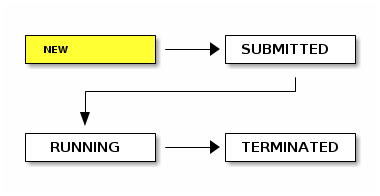
\includegraphics[width=10em]{state-NEW_f7204a67024e58d84956e1cb72fa3f1efb7b5630.png}

  \textbf{NEW} is the state of ``just created'' Application objects.

  The Application has not yet been sent to the Grid: it only exists
  locally.
\end{frame}
\begin{frame}
\frametitle{Application lifecycle: state SUBMITTED}
\label{sec-9}


  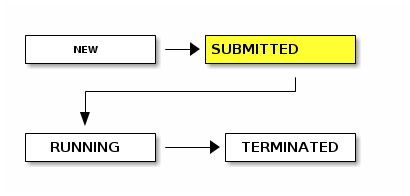
\includegraphics[width=10em]{state-SUBMITTED_ca4e98e5ac36c4ab598d3dd313597f0557206797.png}

  \textbf{SUBMITTED} applications have been successfully queued to a remote
   execution cluster.

   Local Python object has a reference to the remote ``job ID''.
\end{frame}
\begin{frame}
\frametitle{Application lifecycle: state RUNNING}
\label{sec-10}


  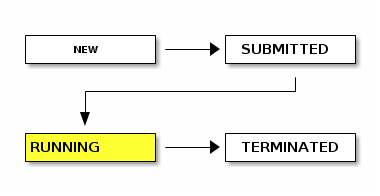
\includegraphics[width=10em]{state-RUNNING_a404c5066c531b1cff0eb57d014cd99da9472404.png}

  \textbf{RUNNING} state happens when the computational job associated to an
   application starts executing on the remote cluster.

   This transition happens independently of GC3Libs; we can only
   monitor progress.
\end{frame}
\begin{frame}
\frametitle{Application lifecycle: state TERMINATED}
\label{sec-11}


  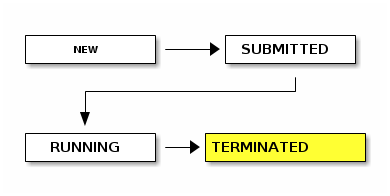
\includegraphics[width=10em]{state-TERMINATED_bd71dc0936d0d6c2ff2cb878d5d8b2b1437ad198.png}

  \textbf{TERMINATED} is when a computational job has finished running,
  for whatever reason.

  The exit code of \textbf{TERMINATED} jobs can be inspected to find out
  whether the termination was successful or unsuccessful, or if the
  program was forcibly ended.
\end{frame}
\begin{frame}
\frametitle{A successful run or not?}
\label{sec-12}

  There's a \emph{single TERMINATED state}, whatever the job outcome.
  
  As with POSIX processes, you have to inspect the exit code and
  signals to determine the cause of ``job death''.
\begin{itemize}
\item If \texttt{os.WIFSIGNALED(app) = False} then job run to completion:
    check exit code!
\item If \texttt{os.WIFSIGNALED(app) = True} then some error occurred before
    end of application code.
\end{itemize}
  
  Grid- and batch-system errors are encoded as ``pseudo-signals''.
  E.g., if \texttt{os.WTERMSIG(app) = 124} then job was killed by remote
  batch system.
  
\end{frame}
\begin{frame}
\frametitle{Core operations}
\label{sec-13}

  Core operations: submit, update state, retrieve (a
  snapshot of) output, cancel job.

  Core operations are \textbf{synchronous}.
  
  Operations are always performed by a \texttt{Core} object.
  \texttt{Core} implements an overlay Grid on the resources 
  specified in the configuration file.
\end{frame}
\begin{frame}[fragile]
\frametitle{Core operations: verb/object interface}
\label{sec-14}

  Get an instance of \texttt{Core}:
\begin{verbatim}
g = Core(read_config_file(path))
\end{verbatim}

  Then you can operate on \texttt{Application} instances:
\begin{itemize}
\item submit: \texttt{g.submit(app)}
\item monitor: \texttt{g.update\_state(app)}
\item fetch output: \texttt{g.fetch\_output(app, dir)} (starts working as soon as
    application is RUNNING)
\item cancel job: \texttt{g.kill(app)}
\item free remote resources: \texttt{g.free(app)}
\end{itemize}
\end{frame}
\begin{frame}[fragile]
\frametitle{Core operations: self-action interface}
\label{sec-15}

  Get an instance of core, then ``attach'' an application to it:
\begin{verbatim}
g = Core(read_config_file())
app.attach(g)
\end{verbatim}

  The application can now operate on itself:
\begin{itemize}
\item submit: \texttt{app.submit()}
\item monitor: \texttt{app.update\_state()}
\item etc.
\end{itemize}

  Combined with state-transition methods, this gives a way to embed
  job control logic in the \texttt{Application} object.

  Think of automatic resubmission if certain conditions are met.
\end{frame}
\begin{frame}
\frametitle{A simple GC3Libs script structure}
\label{sec-16}

\begin{enumerate}
\item Create `gc3libs.Core` instance
\item Create instance(s) of the application class
\item Submit applications
\item Monitor application status (loop)
\item Retrieve results
\item Postprocess and display
\end{enumerate}
\end{frame}
\begin{frame}
\frametitle{What if\ldots{}?}
\label{sec-17}

  Looping is fine with a small number of jobs.

  What if I want to run 10'000 jobs in a session? Do I have to
  loop/wait until all of them are finished?

  What if my box crashes in the middle of the loop?  Do I lose all
  running jobs? 

  What if the proxy expires just in the middle of the loop?
\end{frame}
\begin{frame}
\frametitle{How do I manage authentication with GC3Libs?}
\label{sec-18}

  You don't.

  GC3Libs will check that there is always a valid proxy and
  certificate when attempting Grid operations, and if necessary, renew
  it.  

  GC3Libs provide a specific authentication module, that abstracts on
  the various authentication models.  It can be used to ease/automate
  authentication steps when accessing the Grid.
\end{frame}
\begin{frame}
\frametitle{Persisting jobs}
\label{sec-19}

  GC3Libs provides a simple persistence framework: 
\begin{itemize}
\item save a live \texttt{Application} to disk, return ``persistent ID''
\item load a saved application given its ``persistent ID''
\item delete a saved application
\item list IDs of saved applications (very simplistic! \textbf{your input     needed:} what kind of query/select operations should we support?)
\end{itemize}

  Filesystem-based storage (1 job, 1 file).  But interface is generic,
  could use SQL, \href{http://www.mongodb.org}{MongoDB}, etc.

  Implemented on top of Python's \texttt{pickle} module: it can persist any
  kind of object, not just jobs.
\end{frame}
\begin{frame}
\frametitle{Asynchronous operations}
\label{sec-20}

  The \texttt{Engine} class provides all core operations, 
  with a non-blocking interface.

  Calling core methods on an \texttt{Engine} instance returns immediately to
  the caller; operations are actually executed when you call the
  \texttt{Engine.progress()} method.

  Which you can do in a separate thread, thus achieving
  asynchronous operation.
\end{frame}
\begin{frame}
\frametitle{The \texttt{Engine} class}
\label{sec-21}

  Same programmatic interface as the \texttt{Core} class:
  can drop an \texttt{Engine} instance every time a \texttt{Core} is needed.

  The \texttt{progress()} method will advance jobs through their lifecycle; 
  use state-transition methods to take application-specific actions.
  (E.g., post-process output data.)
  
  An engine can automatically persist the jobs, if you so wish.
  (Just pass it a \texttt{Store} instance at construction time.)
\end{frame}
\begin{frame}
\frametitle{A not-so-simple GC3Libs script structure}
\label{sec-22}

\begin{enumerate}
\item Create `gc3libs.core.Core` instance
\item \emph{Create a `gc3libs.persistence.FilesystemStore` instance}
\item \emph{Create a `gc3libs.core.Engine` instance}
\item \emph{Load saved jobs into it}
\item Create \emph{new} instance(s) of the application class
\item \emph{Let engine manage jobs until all are done}
\item \st{Retrieve results} (the \texttt{Engine} does it)
\item Postprocess and display
\end{enumerate}
\end{frame}
\begin{frame}[fragile]
\frametitle{A not-so-simple GC3Libs script (code)}
\label{sec-23}

\begin{verbatim}
core = Core(read_config_file)
store = FilesystemStore(directory)
apps = [ store.load(jobid) for jobid in open(session, 'r').readlines() ]
for arg in new_args:
  apps += Application(arg, ...)
engine = Engine(core, apps, store)
engine.wait() # call progress() until done
total_global_postprocess()
\end{verbatim}

  This is the \textbf{actual} structure of the GRosetta/GGamess/GRunDB
  scripts! 
\end{frame}
\begin{frame}
\frametitle{Job dependency management}
\label{sec-24}

  An \texttt{Engine} manages all jobs concurrently.
  What if there are inter-application dependencies?

  GC3Libs provides \emph{(untested)} \href{http://en.wikipedia.org/wiki/Directed_acyclic_graph}{Directed Acyclic Graph} support.

  DAGs are created programmatically from Python code.

  Which means, no graphical editor.  But also means you can create
  workflows on-the-fly as your computation proceeds.
\end{frame}
\begin{frame}
\frametitle{Composition of jobs (I)}
\label{sec-25}

  The unit of job composition is called a \texttt{Task} in GC3Libs.

  An \texttt{Application} is the primary instance of a \texttt{Task}.

  However, a single task can be composed of many applications.
  A task is a composite object: tasks can be composed of other tasks.

  Workflows are built by composing tasks in different ways.
  A ``workflow'' is a task, too.
\end{frame}
\begin{frame}
\frametitle{Composition of jobs (II)}
\label{sec-26}

  The \texttt{SequentialTask} class takes a list of jobs and executes them
  one after the other. Subclass and override the \texttt{next()} method to
  determine early exit conditions, or to modify the list dynamically.

  The \texttt{ParallelTask} class takes a list of jobs and executes all of
  them in parallel.  It's done when all jobs are done: there's an
  implicit synchronization barrier at the end.
  
\end{frame}
\begin{frame}
\frametitle{Composition of jobs (III)}
\label{sec-27}

  \texttt{Application}, \texttt{SequentialTask} and \texttt{ParallelTask} are all
  subclasses of the same \texttt{Task} interface.

  So, you can create sequential collections of parallel jobs, parallel
  collections of sequential collections, etc.

  Any DAG can be expressed as composition of these classes.
  And collections can be mutated at run-time.

  An \texttt{Engine} really manages a list of tasks, so we are really
  scripting workflows here.
\end{frame}
\begin{frame}
\frametitle{Well, \emph{almost///}}
\label{sec-28}


  GC3Libs in active development.  We are still experimenting with some
  APIs.  Parts of the code not fully tested.

  Long list of features requests, planned improvements, and bug
  reports. 

  Small team: we work is being prioritized according to requests from
  users, but sometimes it takes quite some time from request to
  implementation.
  
\end{frame}
\begin{frame}
\frametitle{References}
\label{sec-29}

\begin{center}
GC3Pie home page: \href{http://gc3pie.googlecode.com}{http://gc3pie.googlecode.com}

Source code: \texttt{svn co http://gc3pie.googlecode.com/svn}

Mailing list: gc3pie@googlegroups.com

Any questions?
\end{center}
\end{frame}

\end{document}